%*****************************************
\chapter{Staphylococcus aureus}\label{ch:staph}
%*****************************************

\section{Introduction}

The word "Staphilus" derives from the Greek "σταφυλόκοκκος", composed of "staphylé" meaning bundle, and "coccus" meaning grape. This refers to their bundle of grapes-like arrangement. "Aureus" comes from Latin origin meaning golden, which is the golden-orange characteristic color of this bacteria as it is rich in carotenoid pigments. \gls{staph} was discovered in 1880 by Alexander Ogston who noticed a formation of bacteria in pus during a procedure he was performing. Wounds caused by \gls{staph} infections were fatal for most patients until the 1940s when it was discovered that penicillin could cure such infections. But unfortunately, by the end of the century, the penicillin resistance strain became widespread. This led to the development of methicillin, which was a better option to treat infections caused by the bacteria. However, again, the bacteria evolved to be antibiotic resistant, called \gls{mrsa}. Once this strain was characteristic of the hospital, but today is widespread in the general population.

Nearly 30\% of humans are carriers of \textit{S. Aureus} which are usually present in the skin and the upper respiratory tract. Males have a higher prevalence, but the bacteria can also be found specifically in the lower reproductive tracts of females. Under normal circumstances the bacteria are harmless, but they can cause a wide range of diseases which will be discussed later, ranging from minor skin diseases such as pimples or follicles the most common ones, to life-threatening ones such as pneumonia, endocarditis, and sepsis. Is in the top five most common intrahospital infections and is the most common cause of wound infection after surgery, causing around 500.000 hospital infections in the US alone, of which 10\% end up in death related to such infections.

In the forthcoming chapter, the primary attributes of this bacterium will be described, alongside a comparative description of its likeness to other pathogens and to what makes it unique.

\section{Microbiology introduction}

There are 5 pathogenic agents for humans. Four of them are microbes (viruses, bacteria, fungi, and parasites) and the last one is called prions.

\begin{itemize}

\item 
\textbf{Prions} are misfolded proteins capable of making other well-structured proteins also misfold, triggering a chain reaction in the organism. Generally, they provoke neurodegenerative diseases in humans and are transmitted via ingestion of animal corpses that already contain the protein. A well-known example of this in cattle would be \gls{bse}, commonly known as mad cow disease, which spreads to humans in the form of \gls{vcjd}, which is mainly caused by feeding ground animal carcasses to cows. There's no effective treatment for prion diseases and the only prevention against it is to avoid contaminated meat. Only the complete denaturation of the protein can destroy a prion.

\item 
\textbf{Viruses} characterize for needed a host to inject their genetic profile to reproduce. Once this is done, the viral genetic material merges with the host DNA, forcing the replicating mechanism of DNA to create more copies of the virus. There is a huge range of diseases caused by viruses such as the common cold or AIDS, with also many types of methods of transmission. Treatments generally consist of either a vaccine that teaches the immune system how to recognize the virus before it replicates too much, or antiviral drugs that drop fake DNA blocks that get incorporated into the virus genome preventing further replication.

Neither prions nor viruses are considered to be alive, which is why we refer to viruses as particles and not microbes.

\item 
\textbf{Fungal} infections are likely to be transmitted via inhalation, ingestion, or direct surface contact; and rarely directly from person to person. Diagnosis of fungal infection is relativity easy as only 4 non-opportunist fungi are known to be able to actively infect humans; but in contrast, mycosis is a difficult disease to heal. These diseases typically present as a form of lung or skin infection and range in all possible levels of severity. Mycotoxicosis makes a reference to getting poisoned by fungal toxins, and mycetismus is a reference to getting poisoned by eating the fungi themselves. Neither case has anything to do with infections.


\item 
\textbf{Parasite} may refer to two kinds of organisms. One causes parasitic infections, and the other simply feeds from the host resources but does not necessarily cause diseases or discomfort. Many parasites are not microscopic despite being classified as microbes. Parasites are generally transmitted via contact with parasite reservoirs such as food, water, insects, animals, or feces.

The three main types of parasites are Protozoa single-celled parasites which can multiply inside the host, Helminths which are worms, and Ectoparasites which typically live outside of the host such as lice, fleas, or mosquitos. Common diseases caused by parasites are malaria, Changas, toxoplasmosis, acanthamoebiasis, or trichomoniasis. Symptoms of parasitic infections can include diarrhea, fever, fatigue, weight loss, and skin rashes. Treatment for parasites can involve medications such as antiparasitic drugs or antibiotics.

\item 
\textbf{Bacteria} are usually single-cell organisms. \textit{S. Aureus} generally behaves as a commensal bacteria in the skin and upper respiratory tract body doing no harm, but under certain circumstances, it can become a pathogenic bacteria. Let's explore further the characteristics of bacteria and review the \textit{S. Aureus} in context.


\end{itemize}

\subsection{Prokaryote and Eucaryote}

Prokaryotes are unicellular organisms that lack a nucleus encasing the genetic material and membrane-bound organelles. Their genetic material is a circular DNA molecule located in a region called the nucleoid. They are generally smaller in size and have simple structures compared to eukaryotes. However, they have both a cell wall and a cell membrane. This cell wall is made of peptidoglycan. Prokaryotes are unable to perform cellular respiration and don't have any cytoskeleton. \textit{S. Aureus} belongs to this category. 


Eukaryotes, on the other hand, are more complex organisms that have a nucleus enclosing genetic material and various membrane-bound organelles, such as mitochondria, endoplasmic reticulum, Golgi apparatus, and lysosomes. Their genetic material consists of several linear DNA strands contained within the nucleus. They can be unicellular or multicellular organisms. They have a cell membrane, but not necessarily a cell wall (humans do not). Eukaryotes have a cell wall made up of cellulose or chitin.


\subsection{Gram-positive and Gram-negative}
\label{staph:gram-types}

Gram staining is a technique developed by Hans Christian Gram in 1884 which is used to differentiate between bacteria (prokaryotes cells). The first type is called \colorbox{Purple}{\textcolor{white}{Gram-positive}}, which has a simple structure of only one cell wall made of peptidoglycan and teichoic acid, followed by a cell membrane made of a lipid bilayer, lipoteichoic acid, proteins, and carbohydrates. The second type is called \colorbox{Lavender}{\textcolor{white}{ Gram-negative }} and it has an outer cell membrane, followed by a much thinner cell wall, followed by the inner cell membrane.

The space between membranes is denominated the intermembrane space or periplasm. Both, the cell wall plus cell membrane in Gram-positive bacteria, and the outer membrane, cell wall, and inner membrane in Gram-negative bacteria are called the cell envelope. Outside the cell envelope, we might find the final layer, the glycocalyx, a shell made of polysaccharides, proteins, and lipids, which come from the surface of a bacterium, plus extracellular debris that adheres to the bacterium. Alternatively, the bacterium might have an "S-layer" (surface layer), a monomolecular layer composed of only one or two identical proteins or glycoproteins.

    \begin{figure}[ht]
        \centering
            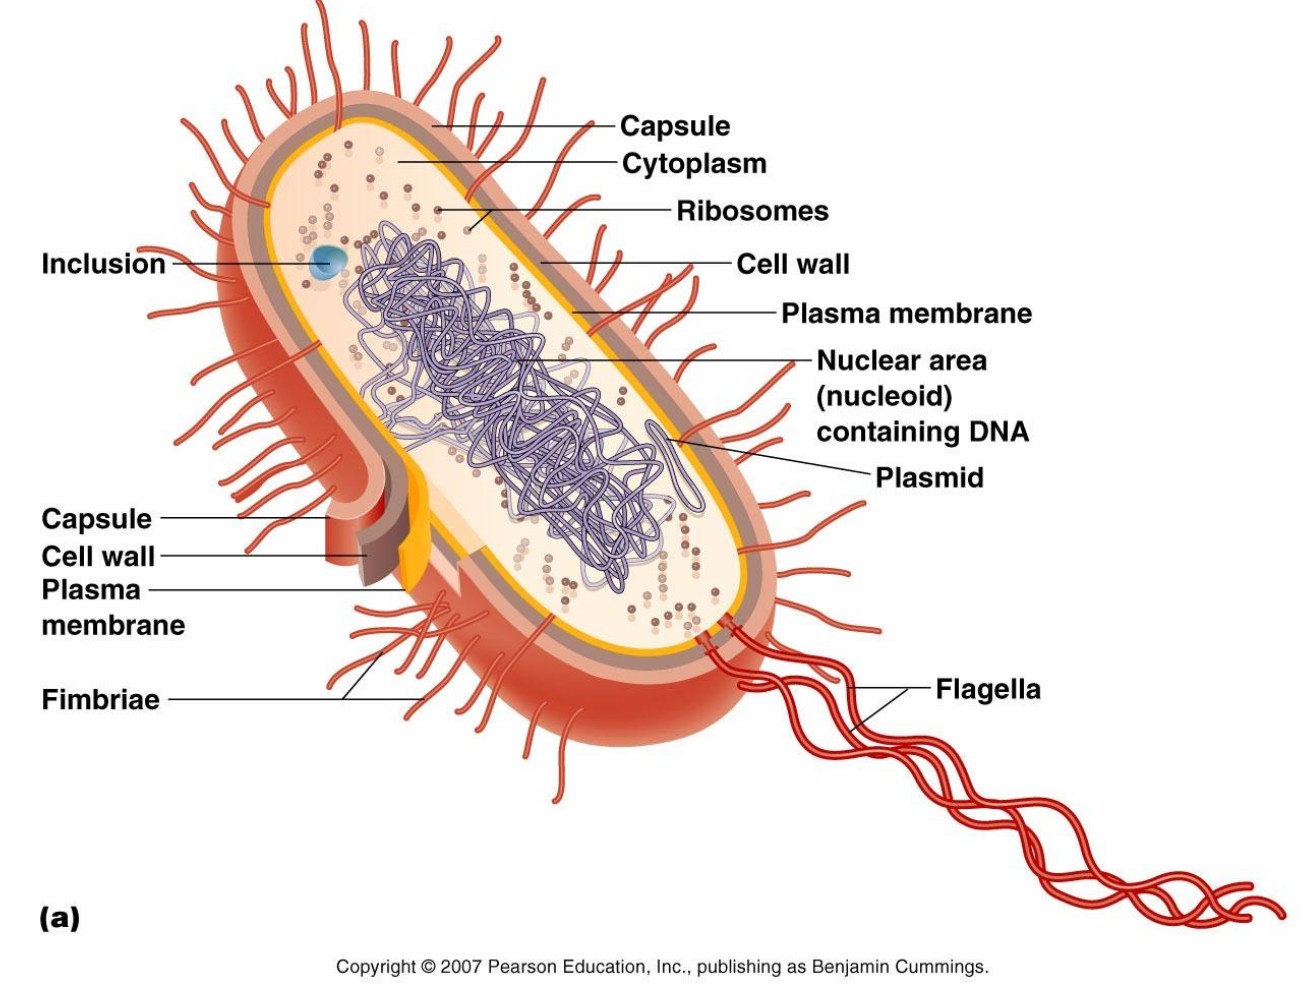
\includegraphics[width=0.7\linewidth]{figures/Staph/bacterialstructure.jpg}
            \caption{Overview of a rod-shaped Gram-positive cell with a capsule. Image property of Pearson Education.}
            \label{figure:capsule}
    \end{figure}

    \begin{figure}[ht]
        \centering
            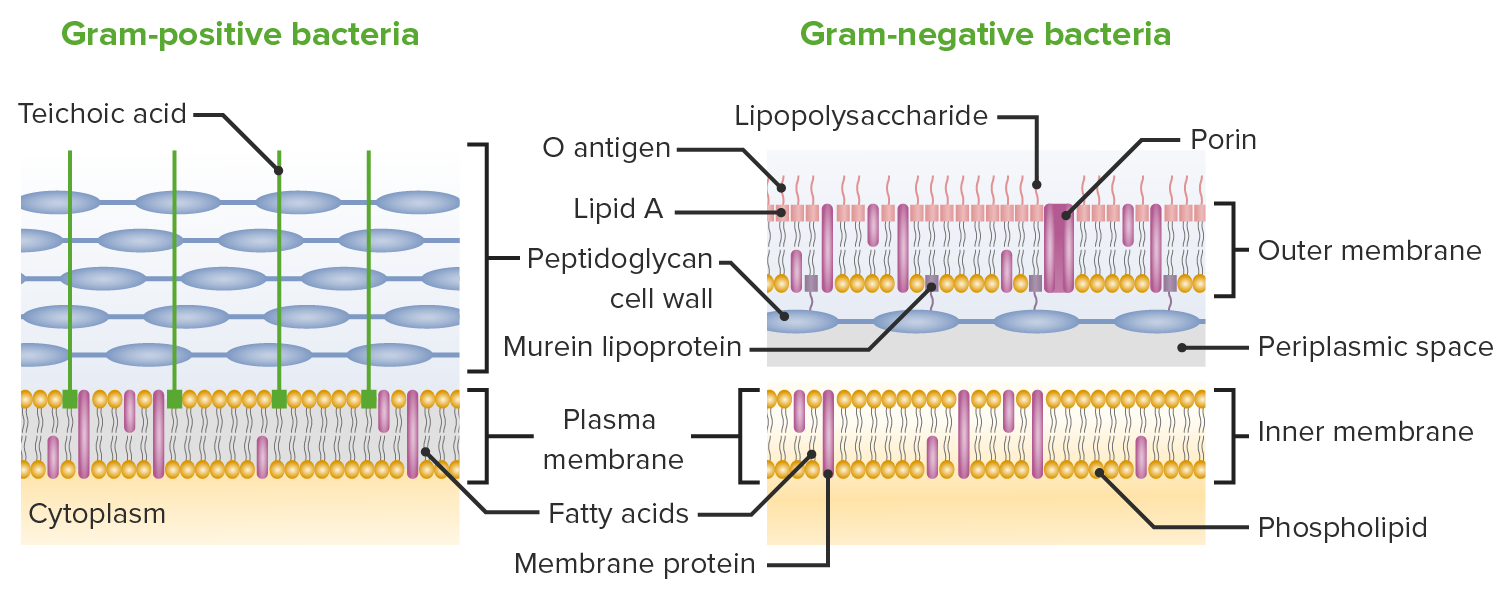
\includegraphics[width=0.7\linewidth]{figures/Staph/Differences-between-gram-positive-and-gram-negative-bacteria-cell.png} 
            \caption{Differences between Gram-positive and Gram-negative cell wall and cell membranes. Reproduced from \url{https://www.lecturio.com/}}
            \label{figure:gram}
    \end{figure}

\subsubsection{Glycocalyx}

Is a gelatinous layer just outside the cell envelope. An irregular gel-like glycocalyx that varies in shape and density is called a slime layer, whereas a distinct more rigid one is called a capsule. In both cases, it serves as a protective function, preventing desiccation, detergents, heat, antibiotics, and phagocytosis. And also in both cases, it contributes to the bacterial structural integrity. 

In addition to protecting the cell from environmental stresses, the glycocalyx particularly the slime layer plays a role in attachment to substrates and host tissue. This is particularly annoying for the host, as the slime layer can help them to stick to tissues or implants and evade the immune system. This is critical for the formation of biofilm, which will be discussed later.

\subsubsection{Outer membrane}
\label{staph:OuterMembrane}

\colorbox{Lavender}{\textcolor{white}{In Gram-negative only.}} The outer membrane contains Porins, which are beta barrel proteins (holes) that open a channel so  specific types of molecules can be transported inside or outside of the cell. Porins also exist in Gram-positive mycobacteria.

It also contains \gls{lps}. These are large molecules that are toxic to humans but are not released from the bacteria towards the host, so they are denominated endotoxin (within-toxin) and are often a synonym of LPS. They are characterized as being very antigenic (polysaccharide O-antigen) and pyrogenic (lipid A) by activating \gls{il1} (fever and inflammation) and \gls{tnfa} (recruiting white blood cells and endothelial activation) Detail about these cytokines will be explained in the inflammation background (chapter  \ref{ch:inflammation}).

\subsubsection{Intermembrane space}

\colorbox{Lavender}{\textcolor{white}{In Gram-negative only.}}. The cell wall is contained within the intermembrane space. So everything that is proper of the cell wall is also in here. Within this space, molecules can accumulate, in particular $\beta$-lactamase, which is very significant in antibiotic resistance.

\subsubsection{Cell wall}

\colorbox{Purple}{\textcolor{white}{In Gram-positive}} bacteria is composed of many peptidoglycan layers, and teichoic acid which is specific to each bacteria species and it allows to bind to fibronectin which will become relevant later on. A peptidoglycan is simply a chain made of peptides and carbohydrates that gives structural support to the cell and gives protection against osmotic damage.

\colorbox{Lavender}{\textcolor{white}{In Gram-negative}} bacteria, it only has a very thin cell wall composed of fewer layers of peptidoglycans.


\subsubsection{Inner membrane}

\colorbox{Purple}{\textcolor{white}{Gram-positive}} bacteria are the only ones that have lipoteichoic acid. It is a regulator of autolytic wall enzymes (prevent the cell from killing itself) and it has specific antigenic properties.

Both \colorbox{Purple}{\textcolor{white}{Gram-positive}} and \colorbox{Lavender}{\textcolor{white}{Gram-negative}} have a phospholipid bilayer, carbohydrates and proteins. In particular, enzymes are responsible for cell wall synthesis and \gls{pbp}. When penicillin binds to PBP, the cell can't make cell walls, and it dies either from collapsing or osmotic damage. Human cells are unaffected by penicillin because eukaryotes cells regulate osmotic damage directly in the cell membrane, and because their structure is supported by their internal cytoskeleton. Bacteria's inner membrane can also protect from osmotic damage, but it relies more on the cell wall for that function.

\subsection{Gram Staining}

The technique consists of three steps:

    \begin{enumerate}
    
        \item Adding crystal violet stain to a bacterial sample. As Gram-positive bacteria have a much thicker peptidoglycan layer they bind to it. Making them more violet-saturated than the Gram-negative. Technically this is all you need, but trying to identify the type by just the violet saturation would render many false positive errors. The next two steps correct this.

        \item Wash out the crystal violet with ethanol, Gram-positives are much harder to wash and the violet color will remain on it while Gram-negatives are decolorized which are difficult to see under the microscope. Thus the next step.

        \item Add a counterstain of Safranin or Fuchsine. Gram-positive will remain violet while Gram-negative will gain a fuchsia color.

    \end{enumerate}

\subsection{Morphology and arrangement}

    \begin{figure}[ht]
        \centering
            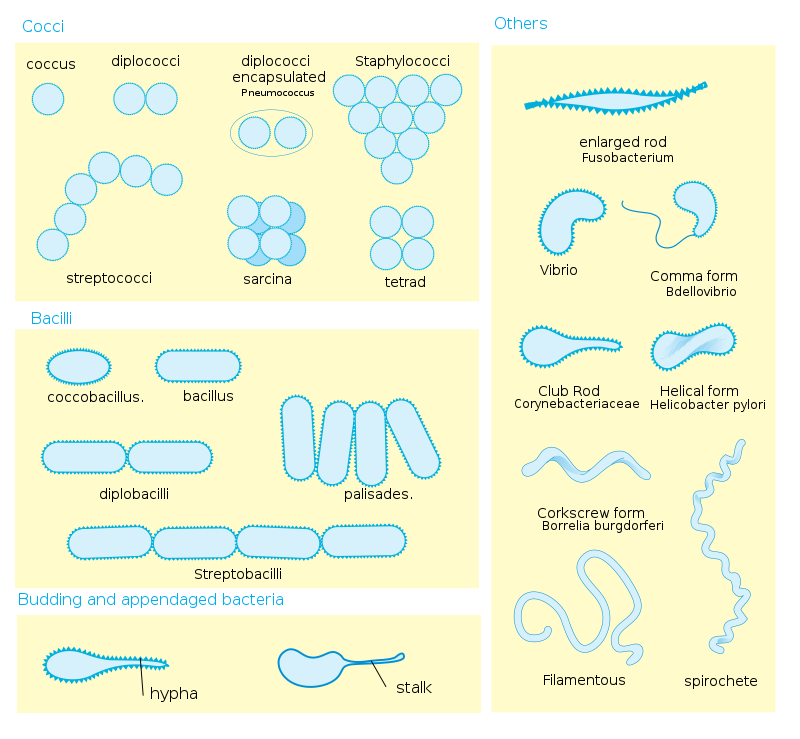
\includegraphics[width=0.7\linewidth]{figures/Staph/Bacterial_morphology_diagram.svg.png} 
        \caption{Different types of bacteria morphologies. Source: Wikimedia.}
        \label{figure:bacteriashapes}
    \end{figure}

Both Gram types can be either cocci (round) or rod-shaped. Rods are also referred to as bacilli, but these are not to be confused with the genus \textit{Bacilli}. Bacteria are italicized in text, as such \textit{Staphylococcus Aureus} is italicized in this thesis. A better example is \textit{Haemophilus influenzae} a bacterium, which shall not be confused with influenza, not italicized, hence a virus. \textit{Staphylococcus} refers to the genus, while \textit{aureus} refers to the species. As the name suggests, \textit{Staphylococcus Aureus} is a cocci bacterium arranged in clusters. Other less common morphologies are included in \ref{figure:bacteriashapes}. 

\subsection{Gram-positive characterization}

\subsubsection{Spore formation}

Rods can be spore-forming or non-spore-forming. Both are sub-categorized into aerobic, and anaerobic. Furthermore, both are divided into Motile and Immotile. They are beyond the scope of this thesis.

Gram-negative bacteria never make spores. However some Gram-positive bacteria can make endospores under some conditions, typically unfavorable environments. This effectively means that they transform from a vegetative state (capable of reproduction) into a spore state, which is a dormant state in which the bacteria are encased and protected by multiple layers of Calcium-Dipicolinic acid. This is the reason why some bacteria are heat resistant, and boiling things, such as your food, can kill some bacteria but not all of them. And why we use autoclaves to sterilize instruments at 121ºC at 15psi for nearly 60 minutes.

\subsubsection{Catalase}

Catalase is an enzyme that catalyzes the conversion of \ch{H2O2} into \ch{H2O} and \ch{O2}. Cocci can be catalase positive forming cocci bundles such as \textit{S. Aureus}, or catalase negative forming cocci rows such as \textit{Streptococci}. A quick test with no microscope, stains, or culture, for bacterial infection is to drop some \ch{H2O2} on it, and if it bubbles (\ch{O2}) it means you have a \textit{Staph} group, and is immune to oxidative burst by neutrophils.

Catalase positive can be divided further using a coagulase test. If the test is positive it means that the sample is a \textit{Staph aureus}. If the test is negative you flood the sample with an antibiotic called novobiocin. If the bacteria die, it means that you have a \textit{Staph epidermis}, but if it is resistant it means that you have \textit{Staph saprophylicus}

Catalase negative are organized in chains, such as the \textit{Streptococcus}, and are classified according to their hemolytic activity. This means they can break down or not red blood cells. Here I will give you some clinically relevant examples.

\begin{itemize}

    \item \textbf{Partial hemolytic ($\alpha$)} Do an optochin resistance test (another antibiotic), if it is sensitive then is \textit{S. Pneumoniae}, if it is resistance you have \gls{vgs}.
    
    \item \textbf{Total hemolitic ($\beta$)} Do another antiobitic resistance test with bacitracin. If it is sensitive you have a \gls{gas} such as \textit{Streptococcus pyogenes}. If it is resistance, you have a \gls{gbs} such as \textit{S. agalactiae}.
    
    \item \textbf{No hemolitic ($\gamma$)} Try to grow it in a \ch{NaCl} solution. If it grows, you have \textit{Enterococci}. If it kills the bacteria, you have \textit{S. Bovis}.
    
\end{itemize}

    \begin{figure}[h!]
        \centering
            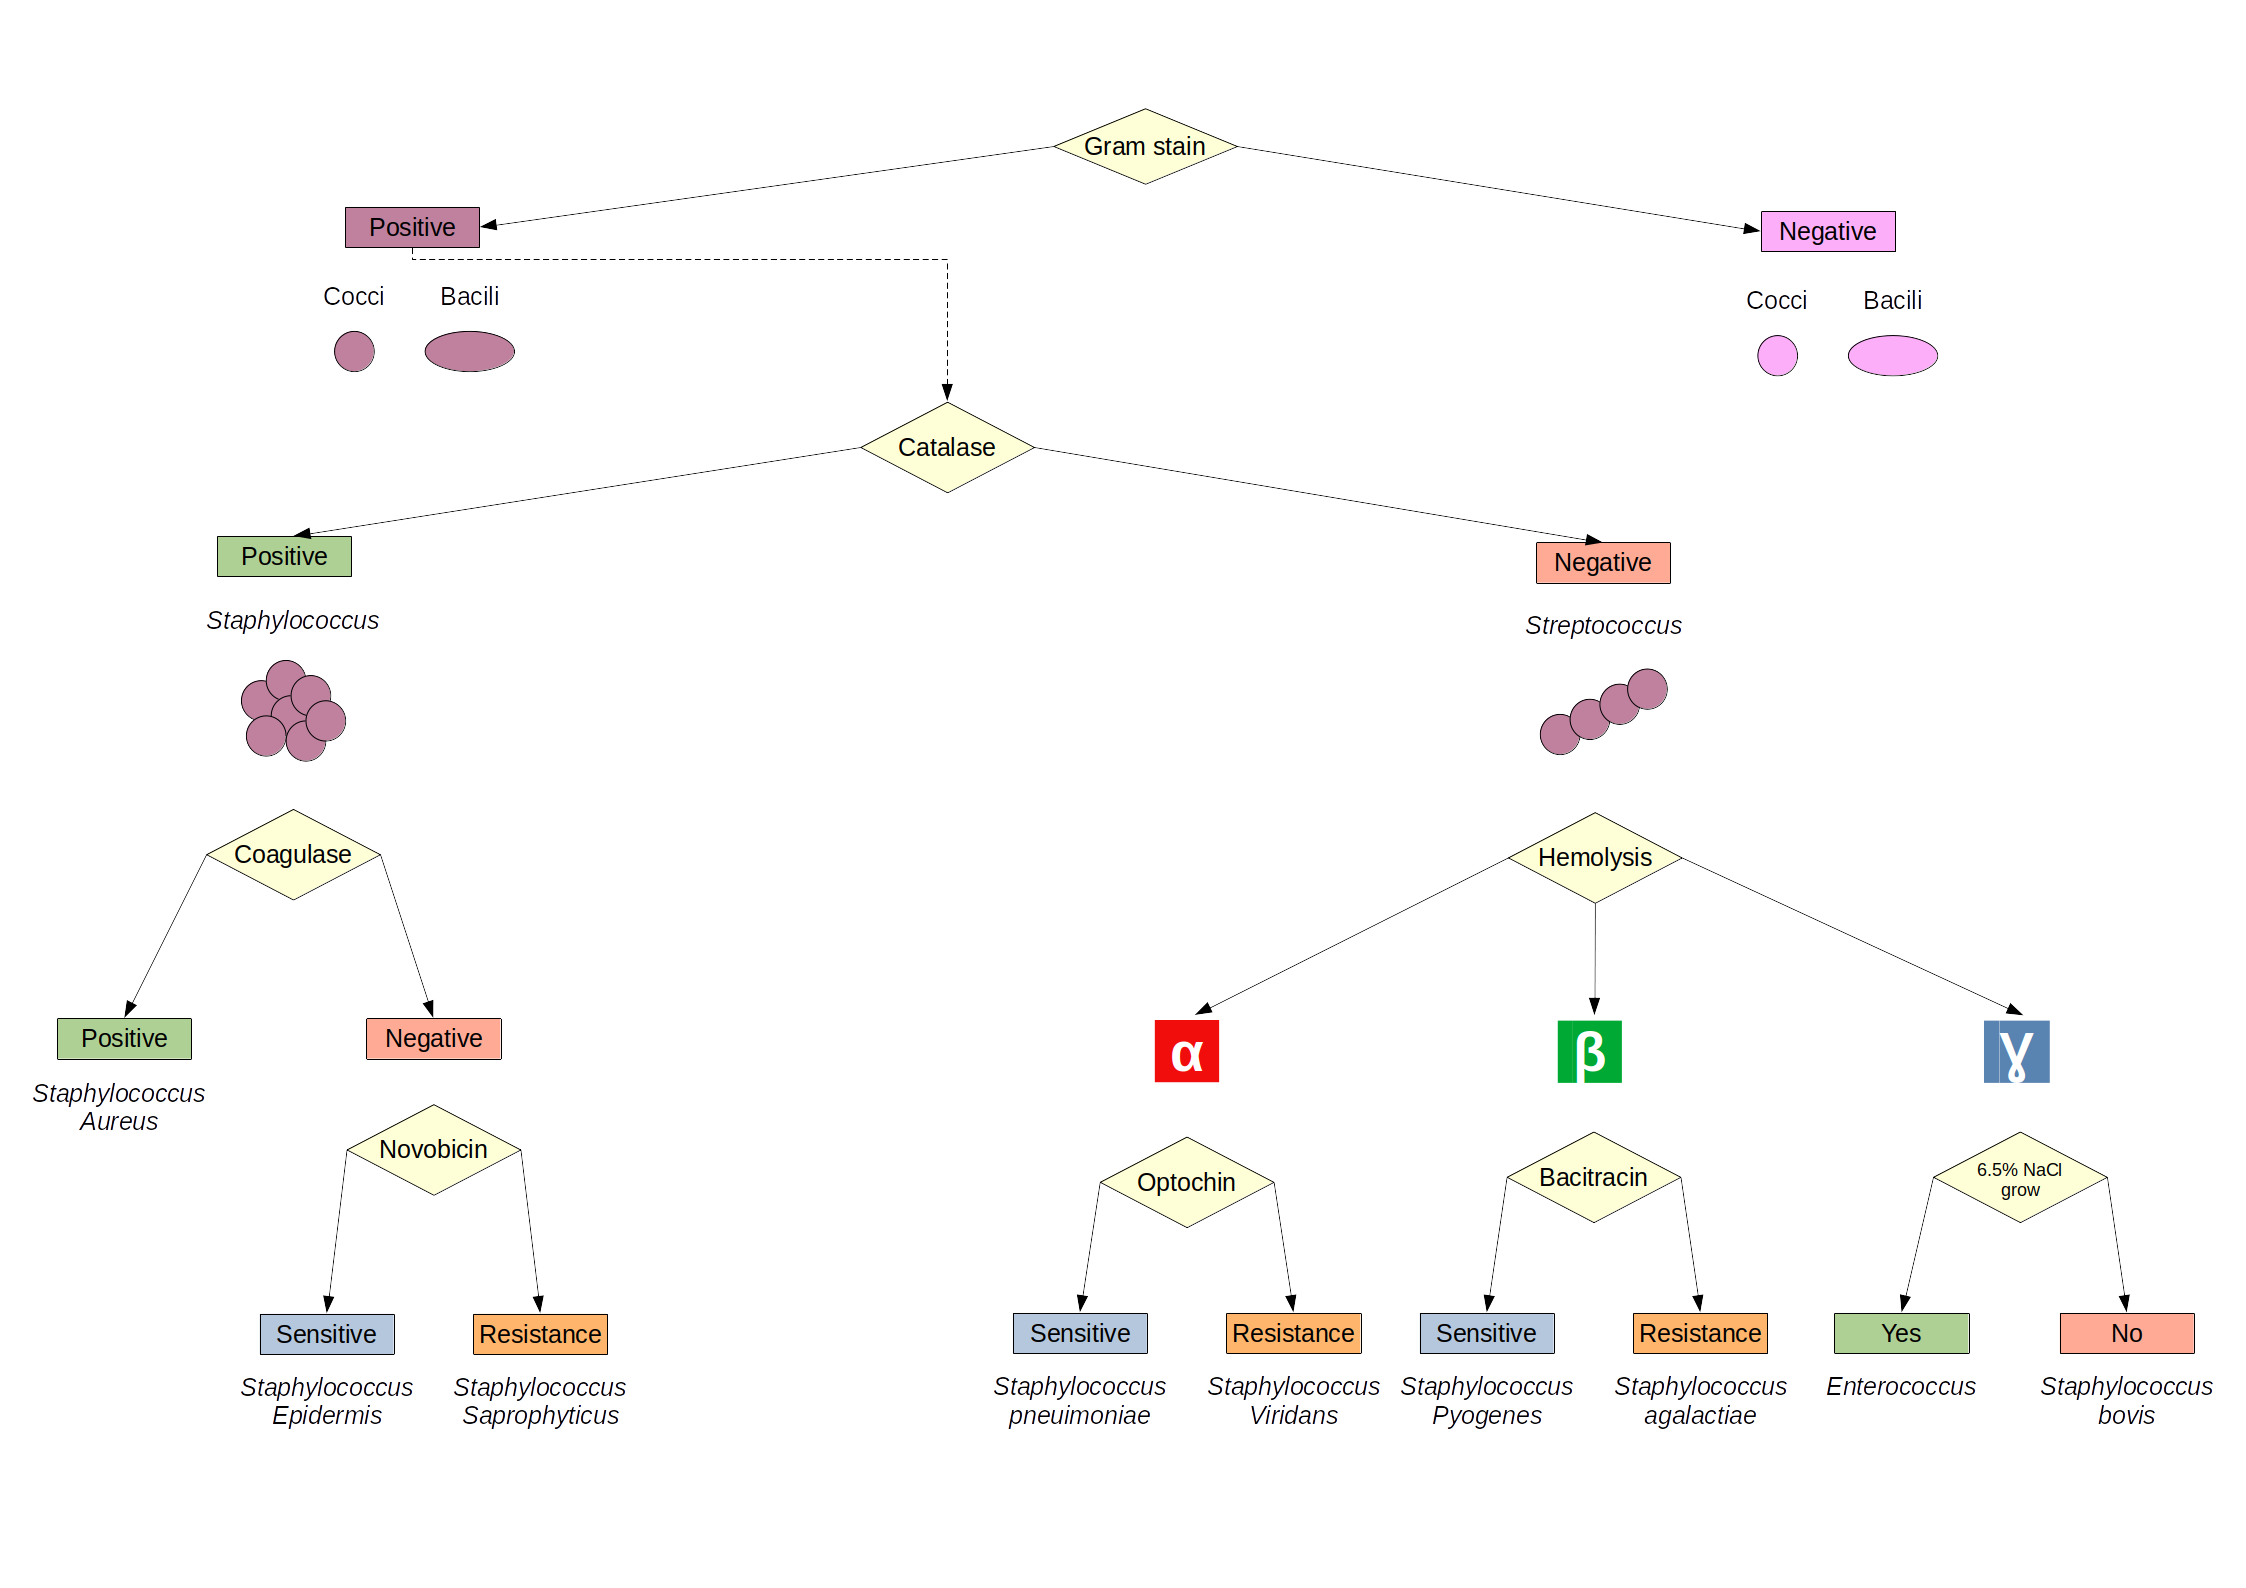
\includegraphics[width=0.9\linewidth]{figures/Staph/Identification.png}
            \caption{Overview of \textit{S. Aureus} identification and other bacteria. Self-made figure.}
            \label{figure:identification}
    \end{figure}

\subsubsection{Fibrin}
\label{staph:Fibrin}

In all cases, all coagulase-positive bacteria lack endospores. "Endo" means with-in, meaning that even though they cannot make their own spores, they can use external tools to make spores. This is the case of Fibrinogen which is found in the human body, and \textit{Staph} uses it to convert it into Fibrin, utilizing coagulase to do so. Effectively, this is employed to hide from the immune system. As a result, coagulase-positive bacteria are highly localized but vary in infection size (folliculitis, abscesses, furuncles, and carbuncles). While coagulase-negative bacteria tend to be widespread (sepsis, cellulitis, necrotizing fasciitis)

Localized bacteria have the advantage that they can be a threat with an incision and drainage as opposed to a widespread infection. The disadvantage is that it exerts much more pressure in the area, especially inside the skull when dealing with brain abscesses.

\section{S. Aureus main characteristics}

\subsection{Bacterial properties}

\textit{S. Aureus} is a prokaryote Gram-positive bacteria capable of growing in both aerobic and anaerobic, and a variety of acidic or based places, although it prefers aerobic and neutral acidic environments such as the skin.

\subsection{Structural components}

\subsubsection{Glycocalix}

The \textit{S. Aureus} can have both a capsule and a slime layer depending on the strain. The \textit{S. Aureus} capsule inhibits phagocytosis as with many other bacteria capsules. Finally, the capsule is prone to contain adhesin proteins which help \textit{S. Aureus} adhere to the epithelium of the mucosa, such as skin, nasopharynx, oropharynx, gastrointestinal tract, and in neonates umbilical stump and peri-anal area. The \textit{S. Aureus} slime layer is prone to forming biofilms. \cite{Parastan2020}

% Lot of sources here: https://www.sciencedirect.com/science/article/abs/pii/S2452014420301539

A biofilm is a community of microorganisms, including bacteria, that stick together on a surface. The biofilm is composed of many layers of cells and \gls{eps}. The EPS is a sticky layer mostly formed by polysaccharides secreted by the bacteria that helps them stick to anything, particularly room surfaces, human tissues, or medical equipment. The EPS also provides a barrier against harmful agents and promotes nutrient exchange and communication between adjacent cells.

    \begin{figure}[h!]
        \centering
            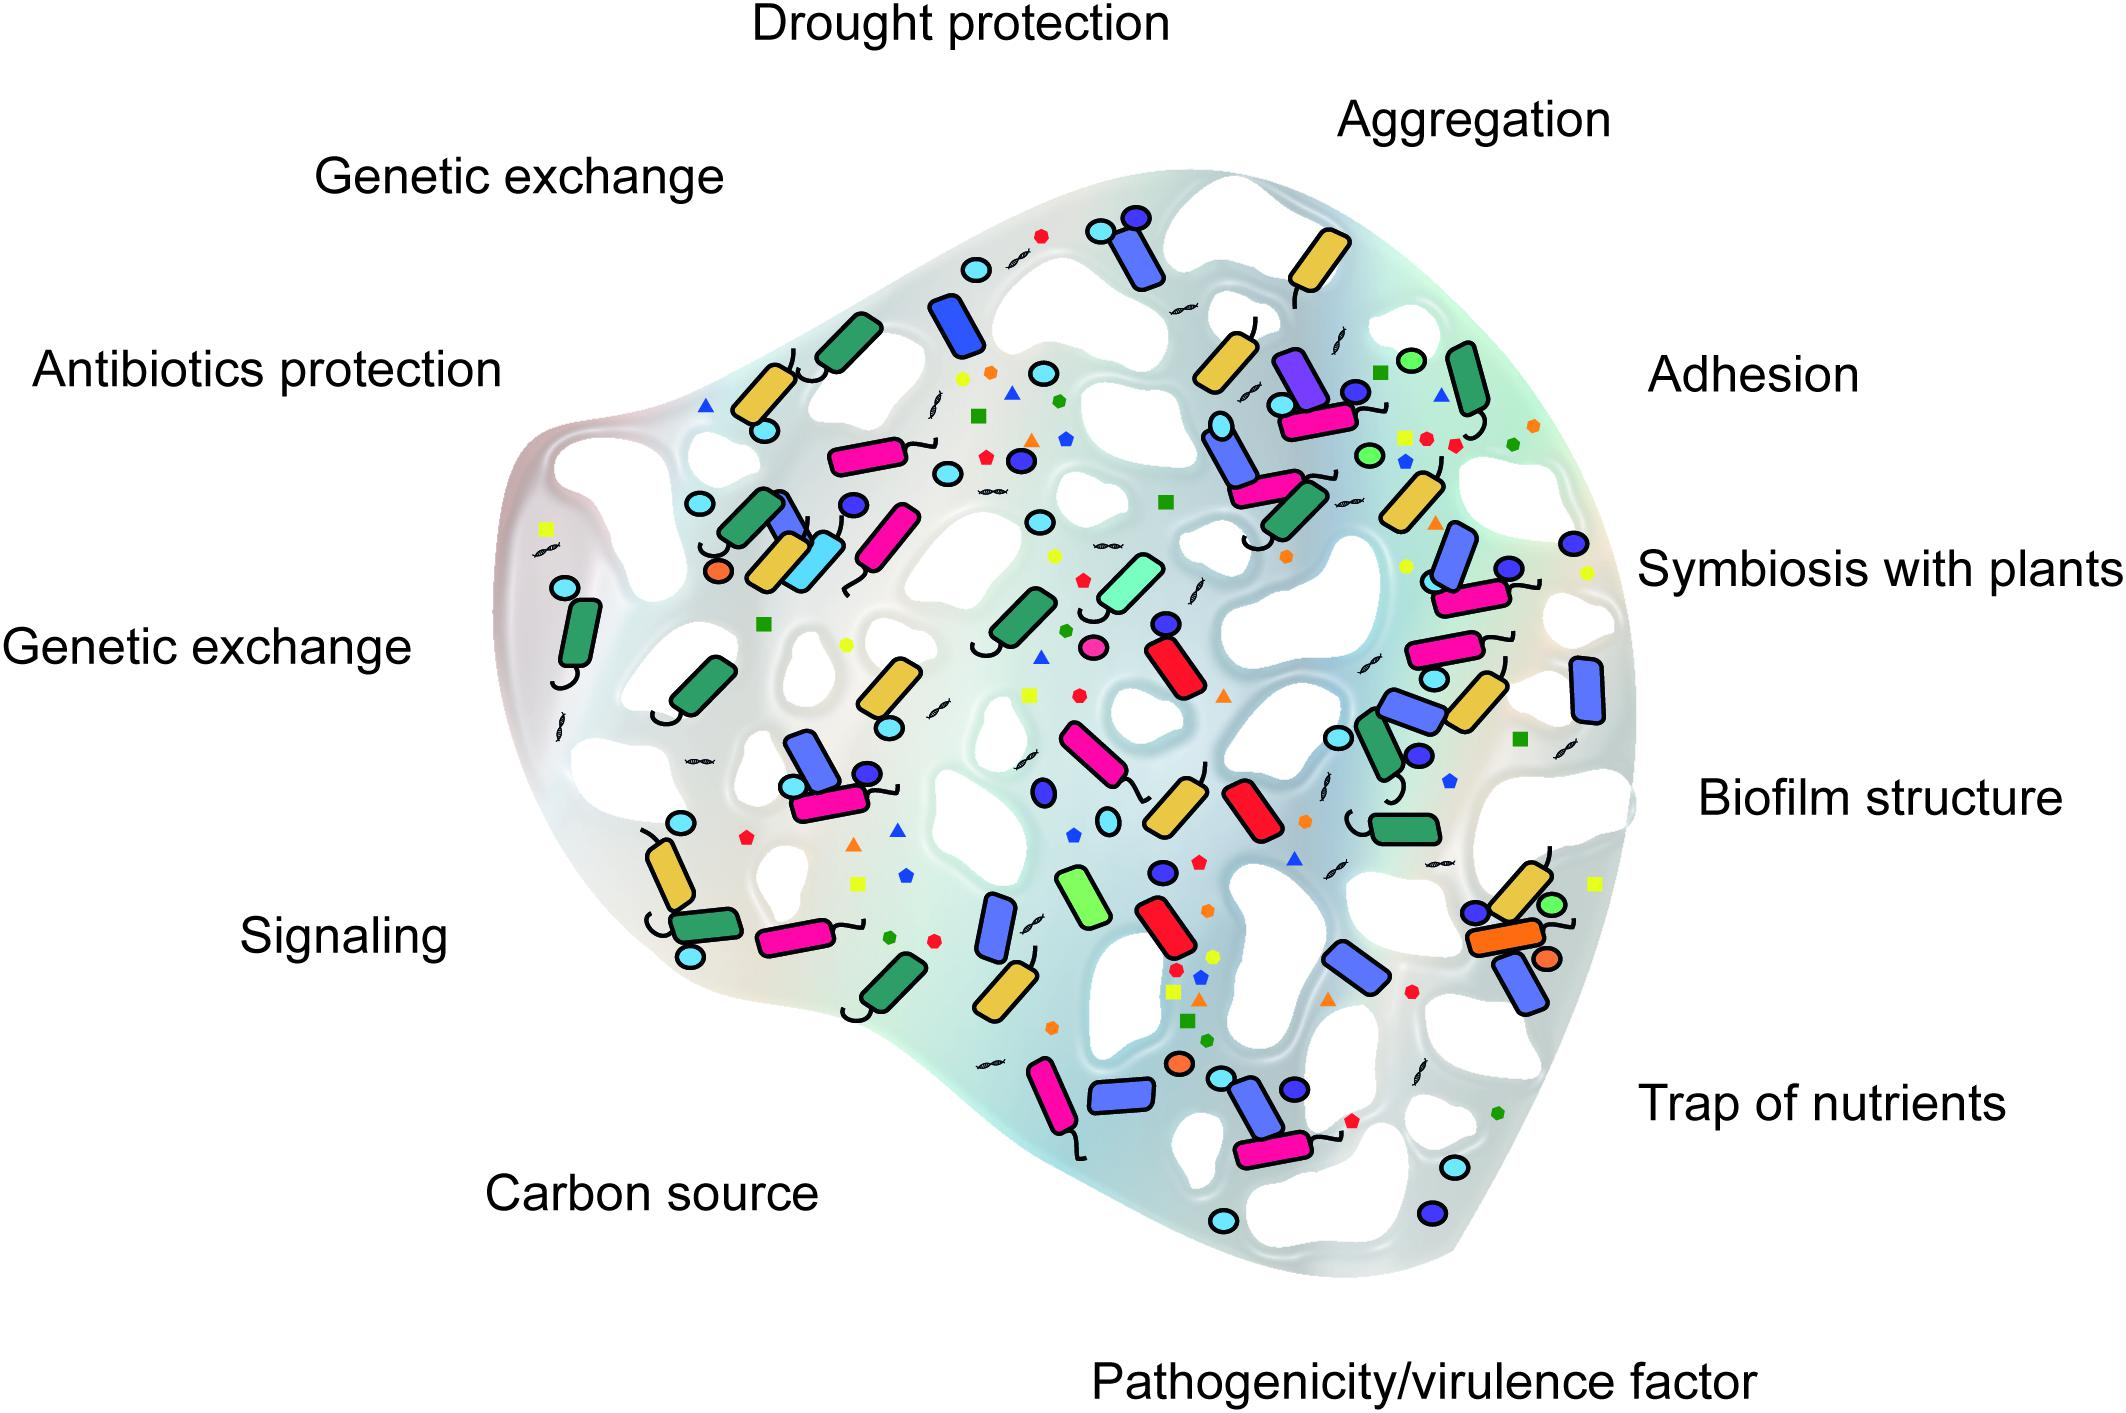
\includegraphics[width=0.7\linewidth]{figures/Staph/fmicb-09-01636-g001.jpg } 
        \caption{Conceptual framework of the functions of microbial extracellular polymeric substances (EPS) in soil. Reproduced from \url{https://doi.org/10.3389/fmicb.2018.01636}}
        \label{figure:EPS}
    \end{figure}

Biofilms are often associated with infections. They are very difficult to detect or treat. The immune system is often unable to break throw the protective exopolysaccharides layer. Antibiotics stay in the blood for a short time and are also unable to penetrate the biofilm, and in the meantime, bacteria hide inside. Biofilms are also the ideal breeding ground for new strains given their protected environment.

\subsubsection{Cell Wall}

The peptidoglycan in the cell wall in the \textit{S. Aureus} is not special. But it provides surface adhesion proteins that have a very special function. They adhere to the peptidoglycan cell wall (bacteria) and at the same time to fibronectin, fibrinogen, collagen, or elastin (human tissue). Technically, it helps the immune system recognize the bacteria which is why are called \gls{mscramm}. But in the \textit{S. Aureus} case, it does the complete opposite:

\begin{itemize}

    \label{stephCellWallSPA}
    \item \textbf{\gls{spa}} arrest antibodies by binding to the constant part of the \gls{igg}, preventing antibody-mediated immune clearance of the \textit{S. Aureus}. Furthermore, this forms an antigen-antibody complex, which activates the classical complement pathway of the complement immune system, wasting it, and leading to hypocomplementemia.

    \item \textbf{Other surface proteins} \textit{S. Aureus} also have \gls{sasc} \cite{Foster2013} \gls{sasg} \cite{Cheng2009} and \gls{sasx} \cite{Josefsson2001}. All of them promote adhesion to desquamated epithelial cells and contribute to biofilm formation.
    
    \item \gls{fnbpa} connect the bacteria with fibronectin and fibrinogen (human parts), which is critical for \textit{S. aureus} virulence. It enables the bacterium to colonize and infect host tissues. In addition, FnBPA contributes to the formation of biofilms. Several small-molecule inhibitors and monoclonal antibodies against FnBPA have been developed and tested in pre-clinical studies approaches for the treatment and prevention of \textit{S. Aureus} infections associated with medical implants.

\end{itemize}

\subsection{Enzymes}

\subsubsection{Coagulase}
\label{stahp:coagulase}

In vertebrates, thrombin converts fibrinogen into fibrin, which later on will form a blood clot aimed to stop hemorrhages. Fibrin also reduces thrombin activity and promotes angiogenesis. All of these are used by \textit{S. Aureus} to its advantage, defining its coagulase abilities.

\gls{clfa} and \gls{clfb} transform fibrinogen into fibrin. They both bind to fibrinogen and promote clotting, forming a shell around the \textit{S. Aureus}, which is the way \textit{S. Aureus}, a coagulase-positive bacterium that lacks endospores as any other, can make something similar to endospores which helps it hide from the immune system on highly localized surfaces. This also serves as an adhesion protein that binds the peptidoglycan cell wall to other surfaces and tissues.

Another feature of \textit{S. Aureus} is its ability to secrete staphylocoagulase and \gls{vwbp}, binding to human thrombin and forming staphylothrombin. Which further promotes fibrinogen to fibrin conversion, forming even more clots.

Interactions of \textit{S. Aureus} and platelets play an important role in the pathogenesis of intravascular infections such as \gls{ie}. A typical feature of \textit{S. aureus} is the ability to generate thrombin activity through the secretion of two prothrombin-activating molecules, staphylocoagulase and \gls{vwbp}, which bind to human prothrombin to form the enzymatically active staphylothrombin complex. The role of staphylothrombin in the interaction between \textit{S. aureus} and platelets have not yet been studied. \cite{Vanassche2012}

\subsubsection{Hyaluronidase}

Hyaluronidases are a family of enzymes that catalyze the degradation of hyaluronic acid. \gls{staph} produce hyaluronidase to obtain carbon from hyaluronan which is abundant in epithelial tissue. Is speculated that \gls{staph} uses Hyaluronidases to destroy the polysaccharide in cells, making it easier to infiltrate in the host.

\subsubsection{Staphylococcal Fibrinolysin}

It is a powerful fibrinolytic enzyme that helps the bacterium to dissolve blood clots in order to spread throughout the host. Staphylokinase plays a key role in the virulence of \textit{S. Aureus} by allowing the bacterium to invade and spread through tissues, in particular the formation of abscesses. It also breaks \gls{igg} and \gls{c3b}, inhibiting phagocytosis, and contributing to hypocomplementemia.

\subsubsection{Lipase}

\textit{S. Aureus} produces lipase to digest lipids into fatty acids and glycerol, which later are turned into ATP. Lipids are also a major component of skin (and other tissues), which helps to colonize human skin more effectively. Lipids also happen to be hydrophobics. As such, when added to the biofilm, lipids help to protect the bacteria against antimicrobial agents.

\subsubsection{Nuclease}

\label{staphNuclease}

A nuclease enzyme is used to break down DNA components and is a common beneficial enzyme required for the central dogma of molecular biology. In the hands of \textit{S. Aureus} however, it breaks down the host DNA into its individual components which the bacterium uses as a source for ATP and other common cellular requirements. This is especially important when the bacteria infiltrate parts of the body where resources are scarce.

Neutrophils can commit suicide as a last method of attacking pathogens by projecting their DNA and using it as a net to catch the invader. This is known as \gls{nets}. Nuclase can break down this trap, allowing it to continue infecting the host. Furthermore, this can also damage healthy cells' DNA prompting apoptosis. All combine to contribute to tissue damage and inflammation.

\subsubsection{Collagen adhesin}

\gls{cna} is a protein that facilitate adhesion to collagen-rich tissue \cite{Patti1994} \cite{MURUGAN2010}. Especially important in the biofilm formation for ocular keratitis and septic arthritis.

\subsubsection{Iron-regulated surface protein}

\gls{isda} and \gls{isdb} facilitate the adhesion to desquamated epithelial cells and promote iron acquisition, typically obtained from the effect of hemolysin. It helps with nasal colonization. \cite{Foster2013} \cite{Cheng2009}

\subsection{Toxins}

\subsubsection{Hemolysin}

This leads to the destruction of the red blood membrane, releasing their hemoglobin, which is used as a source of iron, which is essential for bacterial growth. Secondarily, it can aid immunoevasion because the destruction of red blood cells will lead to inflammation. This means that the immune system will divert resources to soften the inflammation instead of fighting the bacteria. Inflammation can further increase blood permeability allowing the \gls{staph} to transverse blood vessels invading different tissues.

\subsubsection{Exfoliative Toxins}

In between skin cells, keratinocytes, there is a protein called desmoglein-1 which attaches them together packing the skin tight. Exfoliative toxins will damage this connection so they can't stay linked together, leading to patches of the skin falling off. This is the reason why Nikolski's sign symptom manifests in some \textit{S. Aureus} related diseases.

\subsubsection{Enterotoxins}

This targets the enterocytes in the \gls{git}, creating pores on them leading to the destruction of the cell membrane. The sodium inside those cells and other electrolytes leak out, making it more difficult for the rest of the GIT to absorb nutrients, which causes diarrhea. This also damages the epithelium cells of the GIT causing gastroenteritis.

\subsubsection{Panton–Valentine leukocidin (PVL)}
\label{staphPVL}

\gls{pvl} creates pores in leukocytes which lead to ions imbalance making the leukocytes die. This leads to inflammation, particularly in the lungs.

\subsubsection{TSST-1}
\label{staphTSST1}

\gls{tsst1} is a toxin which can be released by \textit{S. Aureus}. This toxin acts as a superantigen. Antigen Presenting Cells have \gls{mhc2} that interact with other cells like T-cells via their CD4 protein. TSST-1 acts as a bridge between the two a hyperstimulates their response leading to a cytokine storm of \gls{il1}, \gls{il2}, \gls{tnfa}, and \gls{ifng}. All of these proteins lead to an inflammatory reaction that acts on the skin creating a rash. They also increase capillary permeability causing vasodilation of the blood vessels leading to both hypotension and hypovolemic shock. Finally, they also increase prostaglandins in the hypothalamus, which leads to fever.

\section{Staph diseases}

\gls{staph} is usually harmless and will just colonize the skin and nasopharyngeal track of the host. However, is also an opportunistic bacterium that easily attaches to many tissues and can develop much more serious complications there.

\subsection{What causes the disease?}

\begin{itemize}

    \item \textbf{Bacteria.} This is when a direct bacterial invasion. To diagnose it you need to look for \gls{igg} related to the bacteria or to perform bacterial cultures. When there are too many, it leads to bacteremia. Generally, if you want to treat it, you do it with antibiotics.
    
    \item \textbf{Toxins.} This is when the bacteria produce toxins that affect the host and produce symptoms. To diagnose it you need to look for \gls{igg} related to the toxin, not the bacteria. When there are too many toxins, it leads to toxemia. They do not respond at all to antibiotics, and samples will show no growth in bacterial agar plates.

\end{itemize}

First, we are going to list the diseases caused by the bacteria, and then, the diseases caused by the toxins.

\subsection{Skin lesions and infections}

They are highly localized due to the coagulase factors. The common ones are superficial abscesses and folliculitis (hair infection). If this becomes severe and deep, they will turn into furuncles (multiple and deeper folliculitis). If it becomes worse, they will turn into carbuncles.

Carbuncle is a deeper folliculitis with multiple sinus tracks, usually on the back and neck. If it goes deeper it passes the fat layer of the skin and reaches, muscles, bones, or blood vessels. Reaching the blood vessels means reaching the blood, which goes everywhere, thus spreading the bacteria in multiple organ tissues. It can also generate septic embolisms in which pus is dislodged from the original site transverse the blood and might land in an organ. Septic embolisms can also be generated in the newly infected organs reaching other random organs via blood vessels.

\textit{S. Aureus} is the most common pathogen associated with wound infections and the most isolated bacteria from chronic wound infections \cite{Bhattacharya2015} such as diabetic foot ulcers. Wound infections are also a common source of septic embolism, which might be caused due trauma (dirty injury), or surgical equipment, which might not be completely clean due to the biofilm properties of \textit{S. Aureus} discussed before. Or even not clean at all such as dirty needles reutilization in drug users.

Cellulitis is also a common complication of \textit{S. Aureus}, however, due to the coagulase mechanisms it tends to stay focalized rather than spread, so is more likely that cellulitis is caused by strep bacteria. 

Depending on the severity, abscesses are generally treated with incision and drainage. If it is a severe case, systemic antibiotics. If it is so severe that it reaches the bloodstream then intravenous antibiotics.

\subsection{Catheter associated infections}

When surgical equipment, prosthetics, needles, or catheters are inserted into a patient, they need to transverse the skin layer which is rich in \textit{S. Aureus}. Even if the equipment is completely clean, this may lead to \textit{S. Aureus} being attached to the equipment, forming a biofilm around it, and staying in the bloodstream until the device is removed. At the same time, the biofilm can release bacteria leading to bacteremia in the blood and spreading everywhere else.

\subsection{Pyomyositis}

Pyomyositis is a bacterial infection of the skeletal muscles which, typically results in an abscess. In the case of \textit{S. Aureus}, secondary pyomyositis which is localized is more frequent. Internal imaging such as CT scans or MRI is required to assess the lesion extension.

\clearpage

\subsection{Endocarditis}

Types of bacterial endocarditis are:

\begin{itemize}

    \item \textbf{Acute.} High-virulence organisms are invading and destroying an intact and healthy heart valve. The \textit{S. Aureus} acts in this group.
    
    \item \textbf{Subacute.} Weak bacteria are attacking a weak valve. Examples of these are the \gls{hacek}.
    
\end{itemize}

It should present with a fever, due to the \textit{S. Aureus} \gls{mscramm} and cloths, and with a new murmur due to the patient having a previously healthy valve. Since the bacteria is already in the blood, it can be diagnosed using a blood culture.

\subsection{Lung abscesses}

Similar to endocarditis, \textit{S. Aureus} goes into the blood and lands in the lungs. Usually causing an excessive amount of liquid (pus) to be allocated in the pleural space in the lung (pleural empyema). It causes productive cough, hemoptysis, or even necrotizing pneumonia. Besides the blood culture, it can also be diagnosed by sputum culture.

\subsection{Brain abscesses}

Similar to endocarditis and lung abscesses, \textit{S. Aureus} goes into the blood and lands in the brain, causing meningitis or brain abscesses. Previously we discussed that \textit{S. Aureus} is heavily localized, it doesn't spread but in exchange can increase pressure in the infected area. This is not a problem in places where it has space to grow, such as the skin. But the skull is 100\% pack with no room for anything else which leads to the increase of \gls{icp}.

This leads to any sort of focal neurological symptoms, as well as classical ICP such as morning frontal headache, projectile vomiting, and blurry vision. When doing a lumbar puncture, it might present an increase exit pressure.

\subsection{Osteomyelitis and septic arthritis}

Once again, \textit{S. Aureus} goes into the blood, which goes into the bone, bone marrow, and joints. However, it can also be caused by direct trauma from something dirty that penetrates the skin and reaches the bone, such as a knife or a bullet.

    \begin{figure}[h]
        \centering
            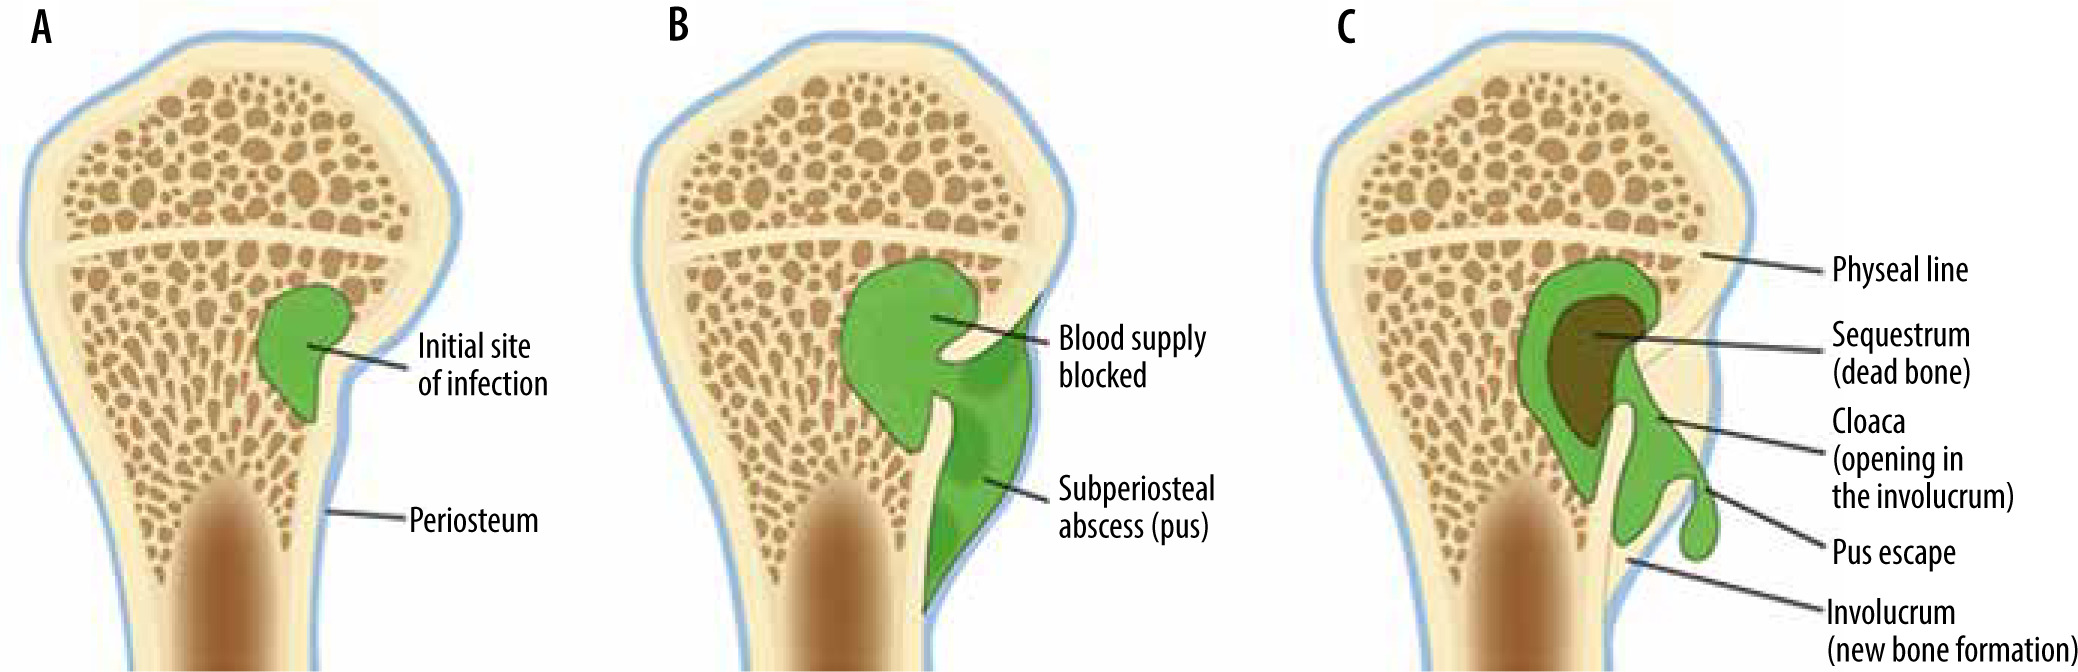
\includegraphics[width=0.7\linewidth]{figures/Staph/PJR-87-46472-g022.jpg} 
        \caption{An artist’s drawing of osteomyelitis progression, subacute to chronic. A) Initial site of osteomyelitis involving the medial aspect of the long bone metaphysis/intraosseous abscess (green). B) The abscess extends through the cortex into the subperiosteal space forming a subperiosteal abscess (shades of green). C) Chronic osteomyelitis with a detached central necrotic bone fragment/sequestrum (brown) within the intraosseous abscess (green) with peripheral new bone formation/involucrum and a cortical and periosteal opening in the involucrum/cloaca allowing the pus to escape. Reproduced from \url{ https://doi.org/10.5114/pjr.2022.113825}}
        \label{figure:osteomyelitis}
    \end{figure}

Is likely to be caused by the metaphysis of the bone due to the stagnated blood circulation in that area, and due to the cartilage blocking the path to the epiphysis. It might lead to septic arthritis (inflammation of the joints), fracture, growth disruption, and vertebral osteomyelitis which can destroy the vertebral cord and develop neurological symptoms. Infections in bones are difficult to treat, which might lead to chronic osteomyelitis, developing into further complications such as sclerosis or the need for amputations.


\subsection{Staphylococcal Scalded Skin Syndrome}

\gls{ssss} is a skin infection. This infection mainly affects patients with weak immune systems, such as babies, children, old individuals, or HIV patients. SSSS is characterized by blistering of the skin similar to a sunburn-like rash, and the skin may feel like it is scalded. It leads to peeling and shedding of the top layer of skin just with mild pressure to the touch (Nikolsky's sign).

It doesn't present any inflammation, no cytolysis, no leukocytosis, and no bacterial growth in cultures because this is not caused by the \textit{S. Aureus}, it is caused by the exfoliative toxins A and B. It heals on its own in about 7 to 10 days and requires only palliative care. However, immunocompromised patients have a mortality rate of 60\%.

\subsection{Ocular infections}

Keratitis is a condition in which the cornea becomes inflamed. This can be caused by introducing \textit{S. Aureus} in the eye, via injury, or dirty contact lenses. Similarly, conjunctivitis can occur. If the infection penetrates deeper into the eye it can turn into endophthalmitis. \cite{MURUGAN2010}

\subsection{Bullous Impetigo}

Is a yellowish crust sore on the skin, normally in areas with skin folds. Is a localized form of \gls{ssss} and is only caused by a specific strain. Is treated with systemic antibiotics such as oral cephalexin. Nonbullous impetigo can be caused by staph or strep bacteria and it can be less severe. In such cases, topical antibiotics can be used.

\subsection{Food poisoning}

If you ever went to a dirty restaurant and ended up vomiting or having diarrhea, is likely that an enterotoxin was the cause. \textit{S. Aureus} have \gls{sea} and \gls{seb}. They are heat resistant and remain even after cooking the food, meaning that you killed the bacteria, but not the toxin. Is likely that the \textit{S. Aureus} ended up in the food due to the chef touching his nose with his fingers, regardless of whether he wore sanitary gloves or not. If food is left uncooked at room temperature it will give \textit{S. Aureus} a better chance to reproduce and create even more toxins. \textit{S. Aureus} also survives in salt.

SEA causes gastroenteritis, it presents no fever and it leads to nausea, vomiting, and watery diarrhea. It usually appears after 5 hours of incubation and resolves itself in less than 24 hours. Treatment includes normal saline for severe cases of dehydration and \gls{nsaids} for severe pain.

SEB cause gastroenteritis and enterocolitis. SEB is a superantigen, which causes the immune system to release a large number of cytokines, which means fever and inflammation. 

\subsection{Toxic Shock Syndrome}

The mechanism described for \gls{tsst1} in section \ref{staphTSST1}, leads to Toxic Shock Syndrome. It usually happens when external objects are left inside the body for too long and do not have an antibiotic coating, such as surgical cures or tampons.

\subsection{Necrotizing Pneumonia}

The mechanism described for \gls{pvl} in section \ref{staphPVL} might kill lung cells which leads to this disease.


\subsection{Antibiotics resistance strains}

\gls{mssa} is vulnerable to various common Methicillin-family antibiotics such as oxacillin, cloxacillin, dicloxacillin, and nafcillin. As the name suggests, also vulnerable to methicillin, which back in time was great because it was a $\beta$-lactamase resistant penicillin. On the bad side, turns out that methicillin also kills the kidneys via interstitial nephritis, which is why methicillin is not used anymore and similar alternatives of the same antibiotics family are used.

As time passed a new strain developed resistance to everything, called \gls{mrsa}. This is due to the bacterium's brand new mecA gene that encodes and produces a \gls{pbp} named PBP2a. This is present in the bacteria cell membrane instead of the original PBP, however, because the structure is different, penicillin (or Methicillin-like antibiotics) can't bind to it anymore. The solution was simple, use Vancomycin to kill the MRSA, especially the hospital-acquired MRSA.

As time passed a new strain came, \gls{vrsa}, which has a brand new van-A gene that alters the peptidoglycan cell wall structure, so the Vancomycin can't prevent cell wall formation anymore. VRSA is treated with Linezolid, daptomycin, telavancin, or ceftaroline. Linezolid is really good but really expensive.

In 2001 there was the first reported case of \gls{lzrsa} \cite{Tsiodras2001}. Then 2006 in China \cite{Jones2007}, 2008 in the US \cite{Mendes2008}, 2006 to 2008 in Japan \cite{IkedaDantsuji2011}, 2008 to 2009 in Spain \cite{Seral2011}, and 2010 in Italy \cite{Mendes2010}. As the reader might have imagined, we already have LZR \textit{Staphylococcus Aureus}. The incidence of LZR staphylococci is still low, but this may change any day due to antibiotic abuse. Limiting hospital stances and antibiotic abuse is critical to limit new antibiotic-resistant strains. LZRSA is currently treated with daptomycin and tedizolid, however, these two antibiotics have severe adverse effects.

\section{Identification}

\subsection{Microscopy}

Direct observation of \textit{S. Aureus} is possible from skin or pus samples. After applying Gram-stain, you should be able to see purple spherical bacteria in cluster form. In bacteremia cases is also possible to observe it blood after culture of the blood sample. Microscopy is a very fast and cheap method as long as the culture is not needed.

\subsection{Culture}
\label{staph:culture}

\textit{S. Aureus} can grow in selective or non-selective media. In selective media, it can trigger false positive results due to the culture being contaminated with other fermentation bacteria, in which case you can add 7.5\% \ch{NaCl} which will kill many other microbes leaving \textit{S. Aureus} alone. It can grow in aerobic or anaerobic and at room temperature. It would grow in around 24 hours and form yellow-orange-ish colonies. It may also present with a green area due to the \textit{S. Aureus} hemolysins partially break down hemoglobin or present a lack of red due complete breakdown of the hemoglobin. Very cheap, and relatively fast.

The culture supernatant can also be tested for the presence of toxins using a biological assay such as a mouse bioassay or a cell cytotoxicity assay.

\subsection{Nucleic Acid Amplification Test}

\gls{naat} consists of amplifying the genetic material of the bacteria, reading the sequencing, and comparing with a database to match \textit{S. Aureus} or any other pathogen. Results are done in about 3 hours but are more expensive.

\gls{pcr} is a commonly known NAAT. This test is highly sensitive and specific and can also be used to detect very low levels of toxins.

\subsection{Biochemical tests}

\subsubsection{Coagulase test}

There are two main methods, slide agglutination test and  tube agglutination test. In both, you get some plasma from the patient or an animal and add the bacteria. If it clumps, it means the bacteria have coagulase enzymes, such as \textit{S. Aureus}. The first method gives you immediate results, while the second one needs to be placed overnight.

    \begin{figure}[h]
        \centering
            \includegraphics[width=0.7\linewidth]{figures/Staph/coagulase_positive_negative_slide.png} 
        \caption{The slide agglutination coagulase test is coagulase positive when clots (clumps) occur with a clear solution in the background (left). The slide coagulase test is coagulase negative when there is a smooth mixture with a milky background (right). Reproduced from \url{ https://bio.libretexts.org/Bookshelves/Microbiology/Microbiology\_Laboratory\_Manual\_(Hartline)/01\%3A\_Labs/1.24\%3A\_Coagulase_Test}}
        \label{figure:coagualaseSlide}
    \end{figure}


    \begin{figure}[h]
        \centering
            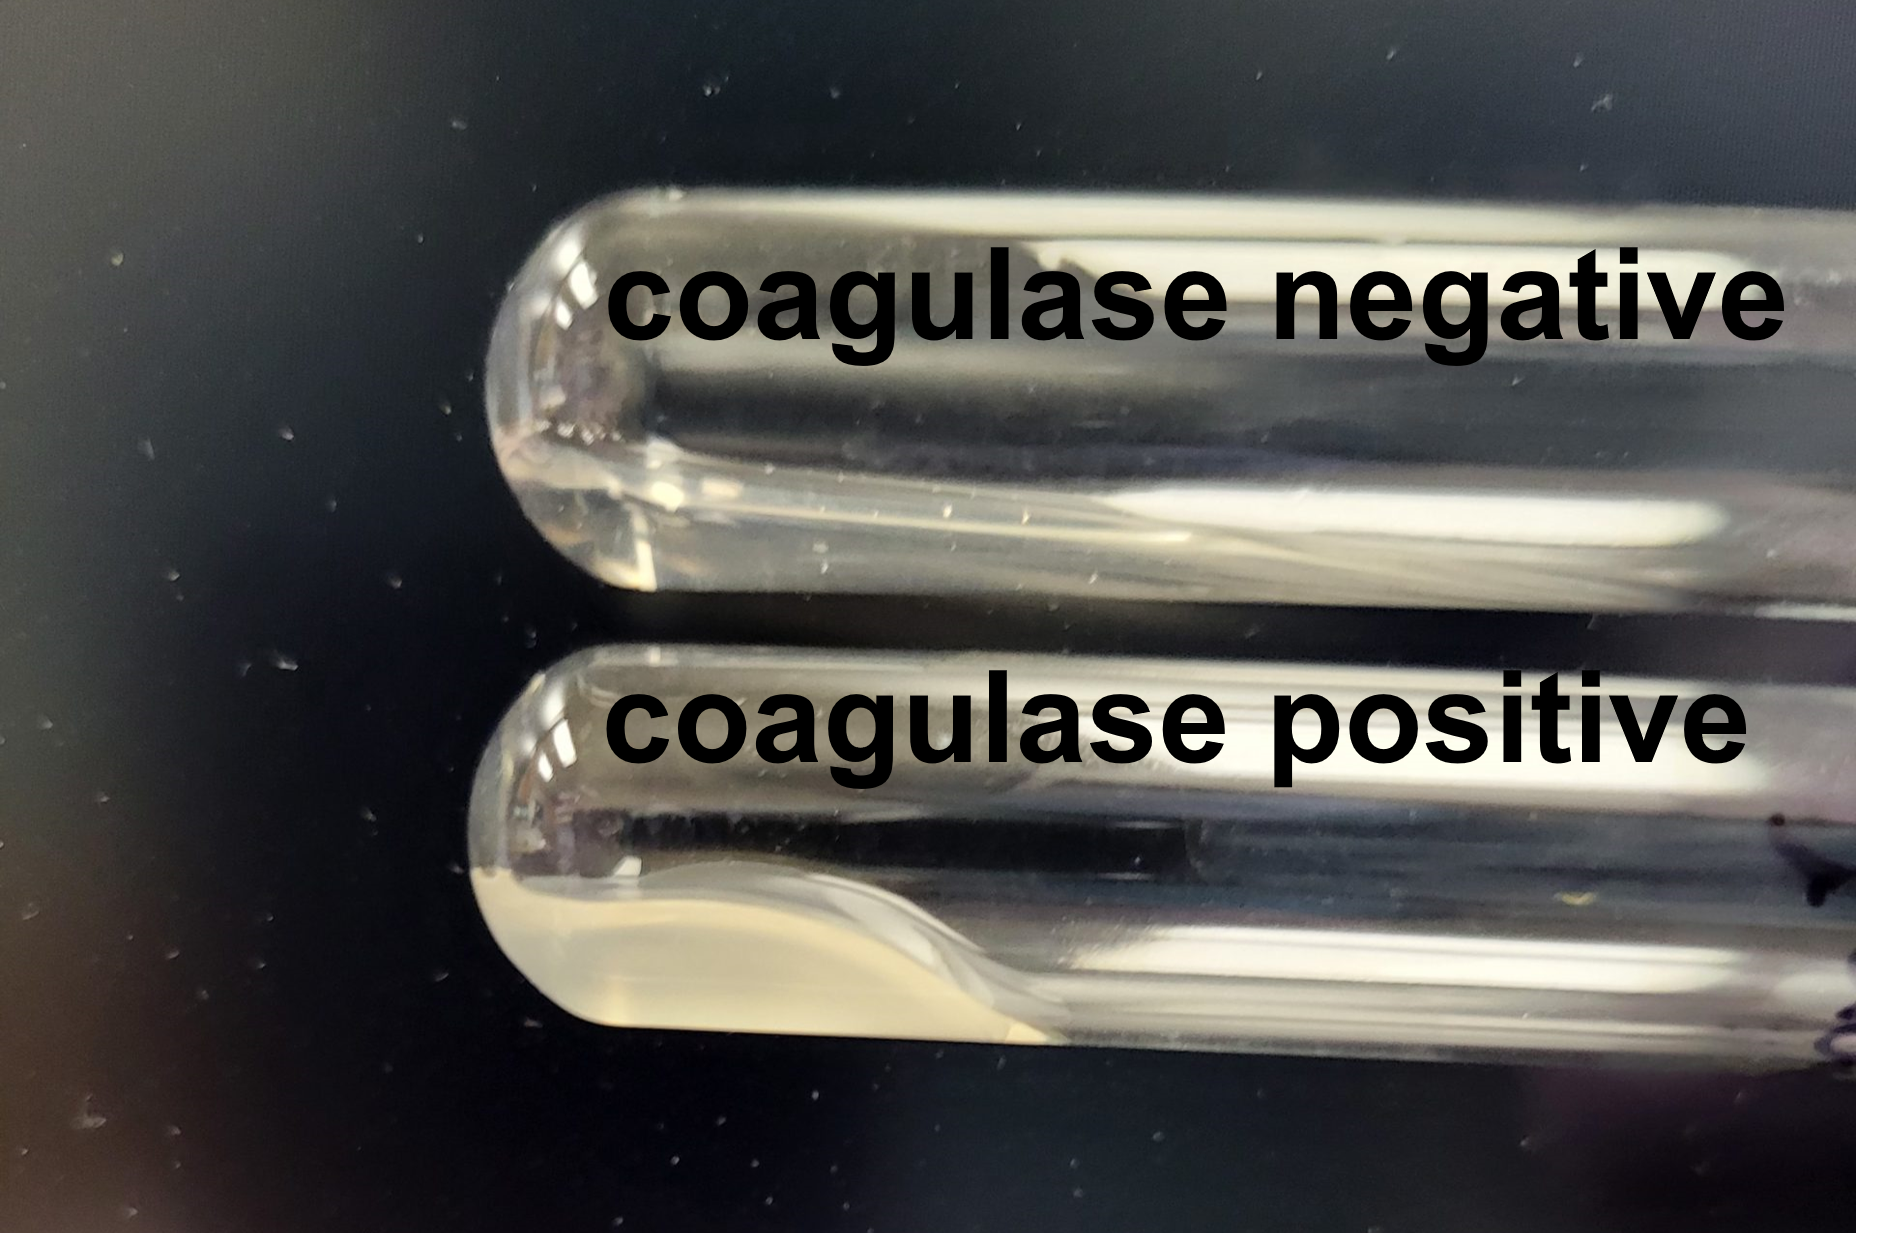
\includegraphics[width=0.7\linewidth]{figures/Staph/coagulase positive negative tube.png} 
        \caption{The tube agglutination coagulase test. When the test tube is tilted, if the fluid is not clumped and does not contain clumps (clotting), the result is coagulase negative (top). When the test tube is tilted, the fluid either exhibits a clump or contains clumps in it (clotting), the result is coagulase positive (bottom). Reproduced from \url{ https://bio.libretexts.org/Bookshelves/Microbiology/Microbiology\_Laboratory\_Manual\_(Hartline)/01\%3A\_Labs/1.24\%3A\_Coagulase_Test}}
        \label{figure:coagualaseTube}
    \end{figure}


Coagulase tests are cheap and quick, but prone to give false positives with other Staphylococcus bacteria such as a novel species the \textit{Staphylococcus Argenteus} \cite{staphArgentusCH}, and false negatives with MRSA strains. There are multiple protocols to add to the test to avoid such misidentifications. \cite{LibreTextStaphID}


\subsubsection{Protein A test}
\label{staph:SPAtest}

The Protein A (section \ref{stephCellWallSPA}) test works by adding a sample from the patient to a plate, usually containing strips coated with antibodies specific to Protein A. If the sample contains \textit{S. aureus}, the Protein A on its surface will bind to the antibodies on the strip, forming a visible line.

\subsubsection{Nuclease test}

\textit{S. Aureus} produce nuclease enzymes (section \ref{staphNuclease}). This test works similarly to the Protein A test. A sample from the patient is added to a plate containing DNA as substrate. After the incubation time period, if the sample contains \textit{S. Aureus} it will break down the DNA leaving empty patches around the bacterial colony.

\subsection{Antibody detection}

An antibody detection test detects the presence of specific antibodies in a person's blood. If the antibodies exist, usually means that a person has developed immunity to the infectious agent.

In the case of \textit{S. Aureus}, it tests for antibodies against the teichoic acids of the bacteria cell wall. If antibodies specific to \textit{S. Aureus} are present in the patient's blood or serum, they will bind to the \textit{S. Aureus} proteins on the plate.

Both Enzyme-linked immunosorbent assay (ELISA) and Immunodiffusion and Western blot can be used to detect specific toxins rather than bacteria.

Generally speaking, antibody detection tests are comparatively quick like NAATs, and much more cheaper. However, antibodies are required to exist in the patient's blood before the test.

\subsection{Mass spectrometry}

Mass spectrometry can't be used to identify the bacteria, but instead can be used to toxins in patient samples by detecting their unique molecular signatures.

\section{Vaccines}

Several vaccines against \textit{S. Aureus} have been developed since 1999 \cite{Parastan2020}, however, due to the bacteria's inmmunoevasive properties, this task has been proven challenging. Furthermore, the safety of these vaccines is still being studied \cite{Xu2017}. Nevertheless, the Staphylococcus aureus 4-Antigen Vaccine vaccine has shown immune Responses up to 36 months \cite{Creech2019}.







